\documentclass[tikz,border=6pt]{standalone}
\usepackage{amsmath}
% =============================================================================
%  PREAMBULE COMMUN DES SCHEMAS DU SUPPORT DE SOUTENANCE (ENSAE, octobre 2026)
%
%  Les schemas sont des VISUELS DE DIAPOSITIVE, pas des figures de donnees : ils
%  prennent donc la palette du gabarit de presentation Nexialog, recopiee de
%  build_soutenance_ppt.py, et jamais celle de style_nexialog.py, qui reste la
%  source unique des couleurs des figures du memoire.
%
%  AUCUN NOMBRE DE RESULTAT N'Y FIGURE. Un nombre dessine dans une image echappe
%  au controle du support, qui verifie chaque nombre de texte contre le rapport.
%  Les schemas portent des symboles et des equations, recopiees du rapport.
%
%  Polices : Segoe UI pour le texte, comme le corps du gabarit ; Latin Modern Math
%  pour les formules, celle du rapport. Chaque schema se dessine A SA TAILLE FINALE
%  sur la diapositive, si bien qu'un corps de 14 pt ici vaut 14 pt a l'ecran.
% =============================================================================
\usepackage{fontspec}
\usepackage{unicode-math}
\setmainfont{Segoe UI}
\setsansfont{Segoe UI}
\setmathfont{latinmodern-math.otf}
\usetikzlibrary{positioning,arrows.meta,calc,fit,backgrounds,shapes.geometric,decorations.pathreplacing}

\definecolor{ardoise}{HTML}{223E55}   % titres et aplats du gabarit
\definecolor{profond}{HTML}{192E3F}
\definecolor{acier}{HTML}{435B6E}
\definecolor{encre}{HTML}{122738}     % texte courant
\definecolor{gris}{HTML}{595959}      % texte secondaire
\definecolor{accent}{HTML}{B10031}    % rouge de marque
\definecolor{clair}{HTML}{F2F2F2}
\definecolor{filet}{HTML}{D9D9D9}

\newcommand{\corps}{\fontsize{14}{17}\selectfont}
\newcommand{\petit}{\fontsize{12}{14.5}\selectfont}
\newcommand{\grand}{\fontsize{16}{19}\selectfont}
\tikzset{
  >={Stealth[length=7pt,width=6pt]},
  bloc/.style={draw=ardoise, line width=0.9pt, fill=white, rounded corners=3pt,
               inner sep=6pt, align=center, text=encre, font=\corps},
  bloc plein/.style={fill=ardoise, draw=ardoise, rounded corners=3pt, inner sep=6pt,
               align=center, text=white, font=\corps\bfseries},
  bloc accent/.style={fill=accent, draw=accent, rounded corners=3pt, inner sep=6pt,
               align=center, text=white, font=\corps\bfseries},
  fleche/.style={->, line width=1.3pt, draw=acier},
  fleche accent/.style={->, line width=1.6pt, draw=accent},
  legende/.style={font=\petit, text=gris, align=center},
}

% -----------------------------------------------------------------------------
%  Schema « du Vasicek a la forme finale avec W, et le seuil K_j » (support de
%  soutenance ENSAE, diapositive de la cascade). Bandeau en trois blocs, environ
%  11,6 x 2,1 pouces. Aucun nombre de resultat. Formules recopiees du rapport :
%   - Vasicek a un facteur et seuil classique : equation (5.1), § 5.1 ;
%   - forme finale : equation (5.3) et sa forme reduite, § 5.3 ;
%   - normalisation de Leontief : equation (5.4), proposition 5.3, § 5.4 et 5.8 ;
%   - seuil de declenchement : equation (5.7), § 5.6.
%  Chaque ligne est posee seule (pas de largeur de texte imposee) : contraintes a
%  une largeur, les formules se coupaient en plein milieu (premier rendu).
% -----------------------------------------------------------------------------
\begin{document}
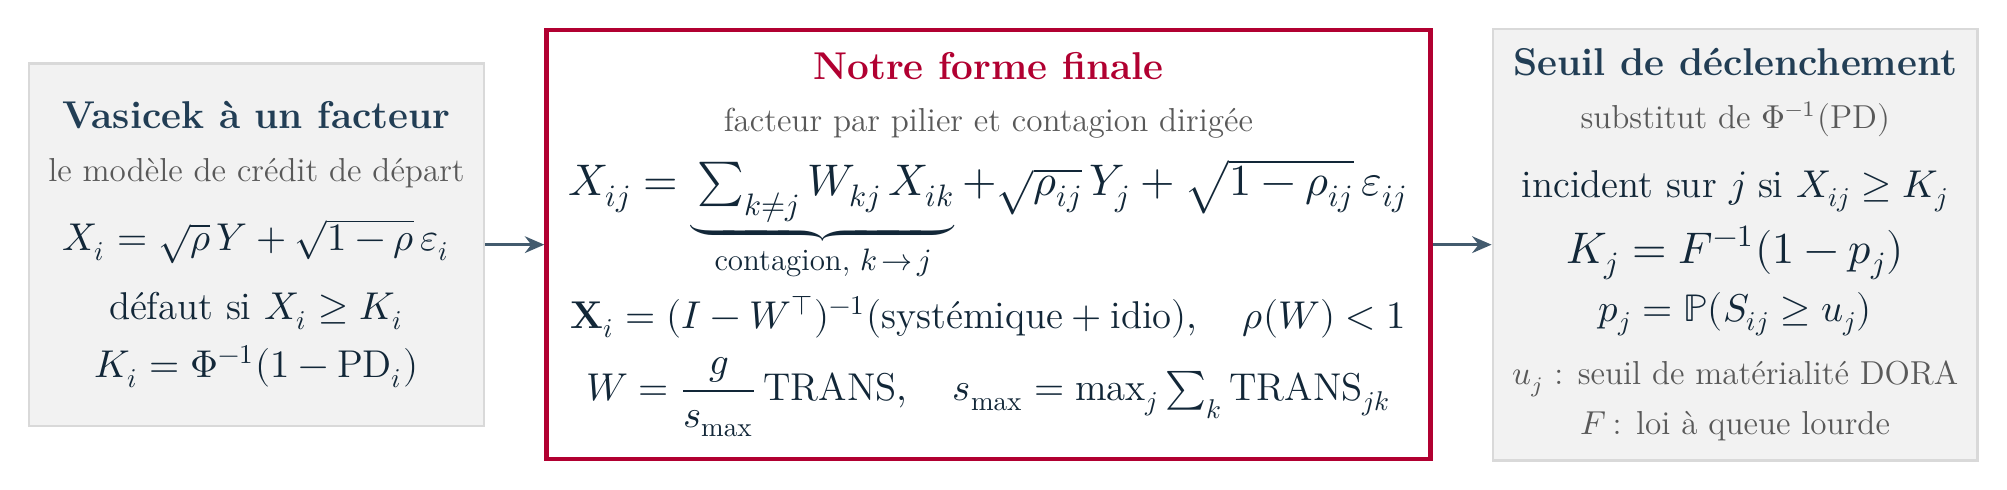
\begin{tikzpicture}[
  boite/.style={draw=filet, line width=0.9pt, fill=clair, inner sep=7pt,
                align=center, text=encre, font=\corps, minimum height=4.6cm},
  finale/.style={draw=accent, line width=1.6pt, fill=white, inner sep=8pt,
                 align=center, text=encre, font=\corps, minimum height=4.6cm},
]
\node[boite] (vas) {%
  {\color{ardoise}\bfseries Vasicek à un facteur}\\[2pt]
  {\petit\color{gris} le modèle de crédit de départ}\\[8pt]
  $X_i=\sqrt{\rho}\,Y+\sqrt{1-\rho}\,\varepsilon_i$\\[8pt]
  défaut si $X_i\ge K_i$\\[4pt]
  $K_i=\Phi^{-1}(1-\mathrm{PD}_i)$};

\node[finale, right=0.75cm of vas] (fin) {%
  {\color{accent}\bfseries Notre forme finale}\\[2pt]
  {\petit\color{gris} facteur par pilier et contagion dirigée}\\[6pt]
  {\grand $X_{ij}=\underbrace{\sum_{k\neq j}W_{kj}\,X_{ik}}_{\text{contagion, }k\,\to\,j}
    +\sqrt{\rho_{ij}}\,Y_j+\sqrt{1-\rho_{ij}}\,\varepsilon_{ij}$}\\[6pt]
  $\mathbf{X}_i=(I-W^{\top})^{-1}(\text{systémique}+\text{idio}),\quad \rho(W)<1$\\[6pt]
  $W=\dfrac{g}{s_{\max}}\,\mathrm{TRANS},\quad s_{\max}=\max_j\sum_k\mathrm{TRANS}_{jk}$};

\node[boite, right=0.75cm of fin] (seuil) {%
  {\color{ardoise}\bfseries Seuil de déclenchement}\\[2pt]
  {\petit\color{gris} substitut de $\Phi^{-1}(\mathrm{PD})$}\\[8pt]
  incident sur $j$ si $X_{ij}\ge K_j$\\[4pt]
  {\grand $K_j=F^{-1}(1-p_j)$}\\[4pt]
  $p_j=\mathbb{P}(S_{ij}\ge u_j)$\\[6pt]
  {\petit\color{gris} $u_j$ : seuil de matérialité DORA}\\[1pt]
  {\petit\color{gris} $F$ : loi à queue lourde}};

\draw[fleche] (vas.east) -- (fin.west);
\draw[fleche] (fin.east) -- (seuil.west);
\end{tikzpicture}
\end{document}
